\subsection{Experiment \rnum{1}: File Loading and Data Processing}


\subsubsection{\acrshort{das} signal heatmaps}

\begin{figure}[!h]
    \centering
    \begin{subfigure}{0.45\linewidth}
        \centering
        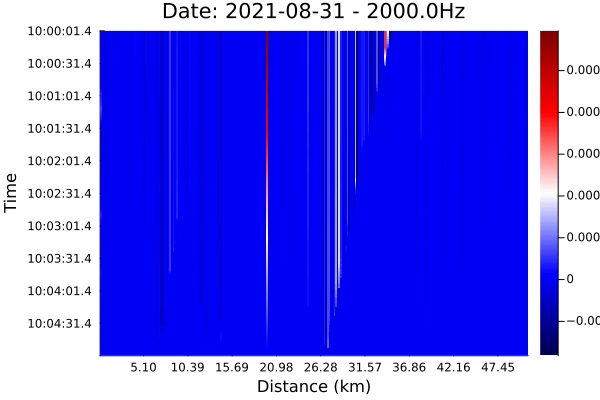
\includegraphics[width=\linewidth]{figures/heatmap_das_test.png}
        \caption{Before}
        \label{fig:dasoutput1}
    \end{subfigure}
    \hfill
    \begin{subfigure}{0.45\linewidth}
        \centering
        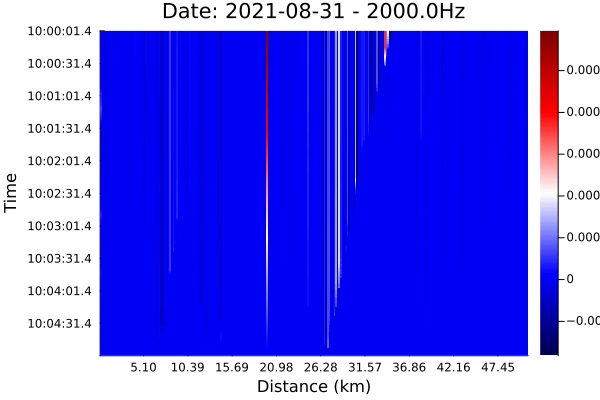
\includegraphics[width=\linewidth]{figures/heatmap_das_test.png}
        \caption{After}
        \label{fig:dasoutput2}
    \end{subfigure}
    \caption{Heatmaps of the processed data before and after resampling}
    \label{fig:dasoutput}
\end{figure}

\begin{figure}[!h]
    \centering
    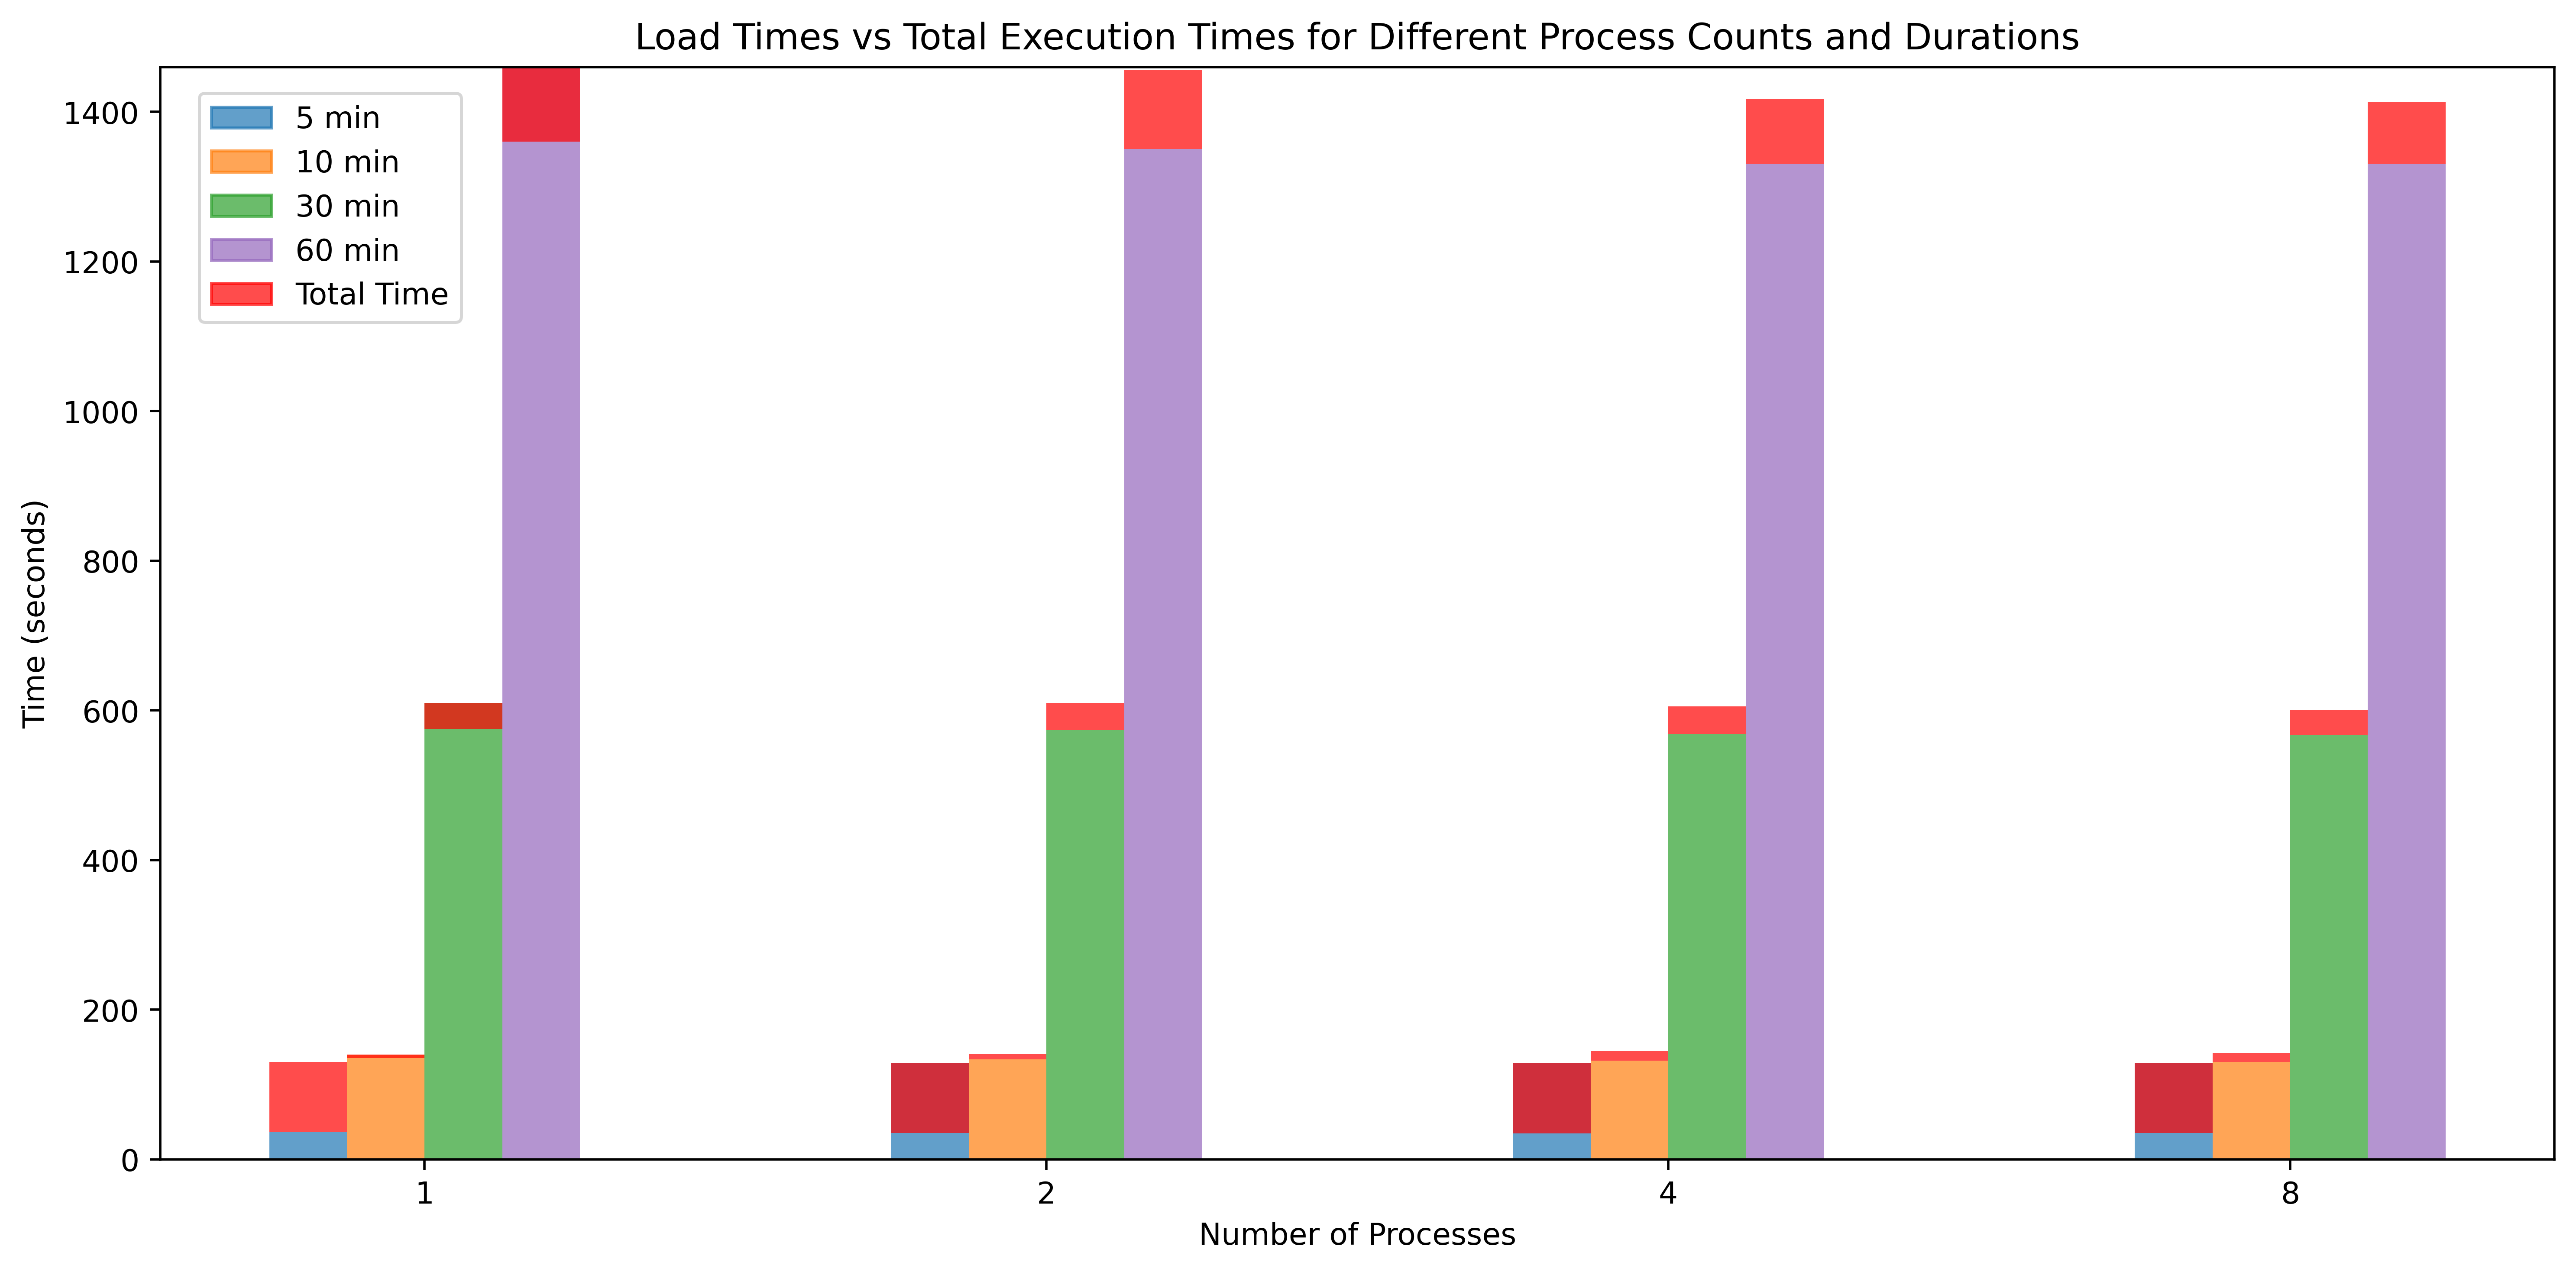
\includegraphics[scale=0.50]{figures/judasex.png}
    \caption{Loading and total processing execution times for different durations and processes. The red bars highlight the total time for processing, while the other bars just show the load times.}
    \label{fig:judasextime}
\end{figure}

Figure \ref{fig:judasextime} highlights the load section's portion. This is the most resource-intensive portion of the program for all processes and file duration except the 5-minute block. 


\begin{figure}[!htbp]
\centering
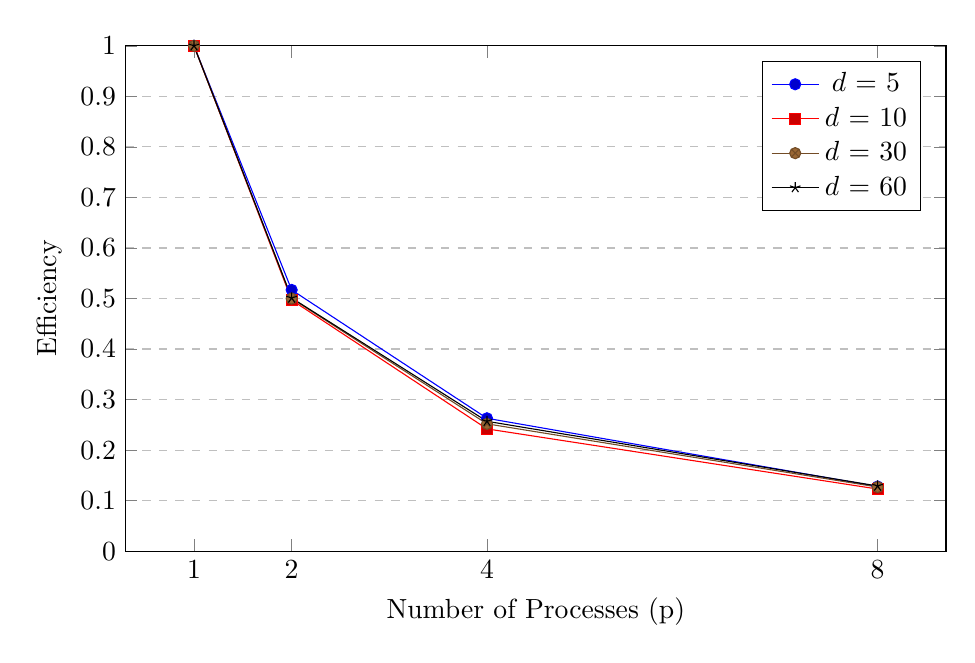
\begin{tikzpicture}
\begin{axis}[
    ylabel={Efficiency},
    xlabel={Number of Processes (p)},
    xticklabels={1,2,4,8},
    xtick={1,2,4,8},
    ytick={0.0, 0.1, 0.2, 0.3, 0.4, 0.5, 0.6, 0.7, 0.8, 0.9, 1.0},
    legend pos=north east,
    ymajorgrids=true,
    grid style=dashed,
    width=12cm,
    height=8cm,
    ymax=1,
    ymin=0,
]
\addplot coordinates {(1,1) (2,0.517) (4,0.263) (8,0.128)};
\addplot coordinates {(1,1) (2,0.497) (4,0.242) (8,0.123)};
\addplot coordinates {(1,1) (2,0.500) (4,0.252) (8,0.127)};
\addplot coordinates {(1,1) (2,0.501) (4,0.257) (8,0.129)};
\legend{$d$ = 5, $d$ = 10, $d$ = 30, $d$ = 60}
\end{axis}
\end{tikzpicture}
\caption{Efficiency for different problem sizes and process counts. $d$ is the loaded signal duration in minutes.}
\label{fig:judasefficiency}
\end{figure}

%\begin{figure}[!h]
%    \centering
%    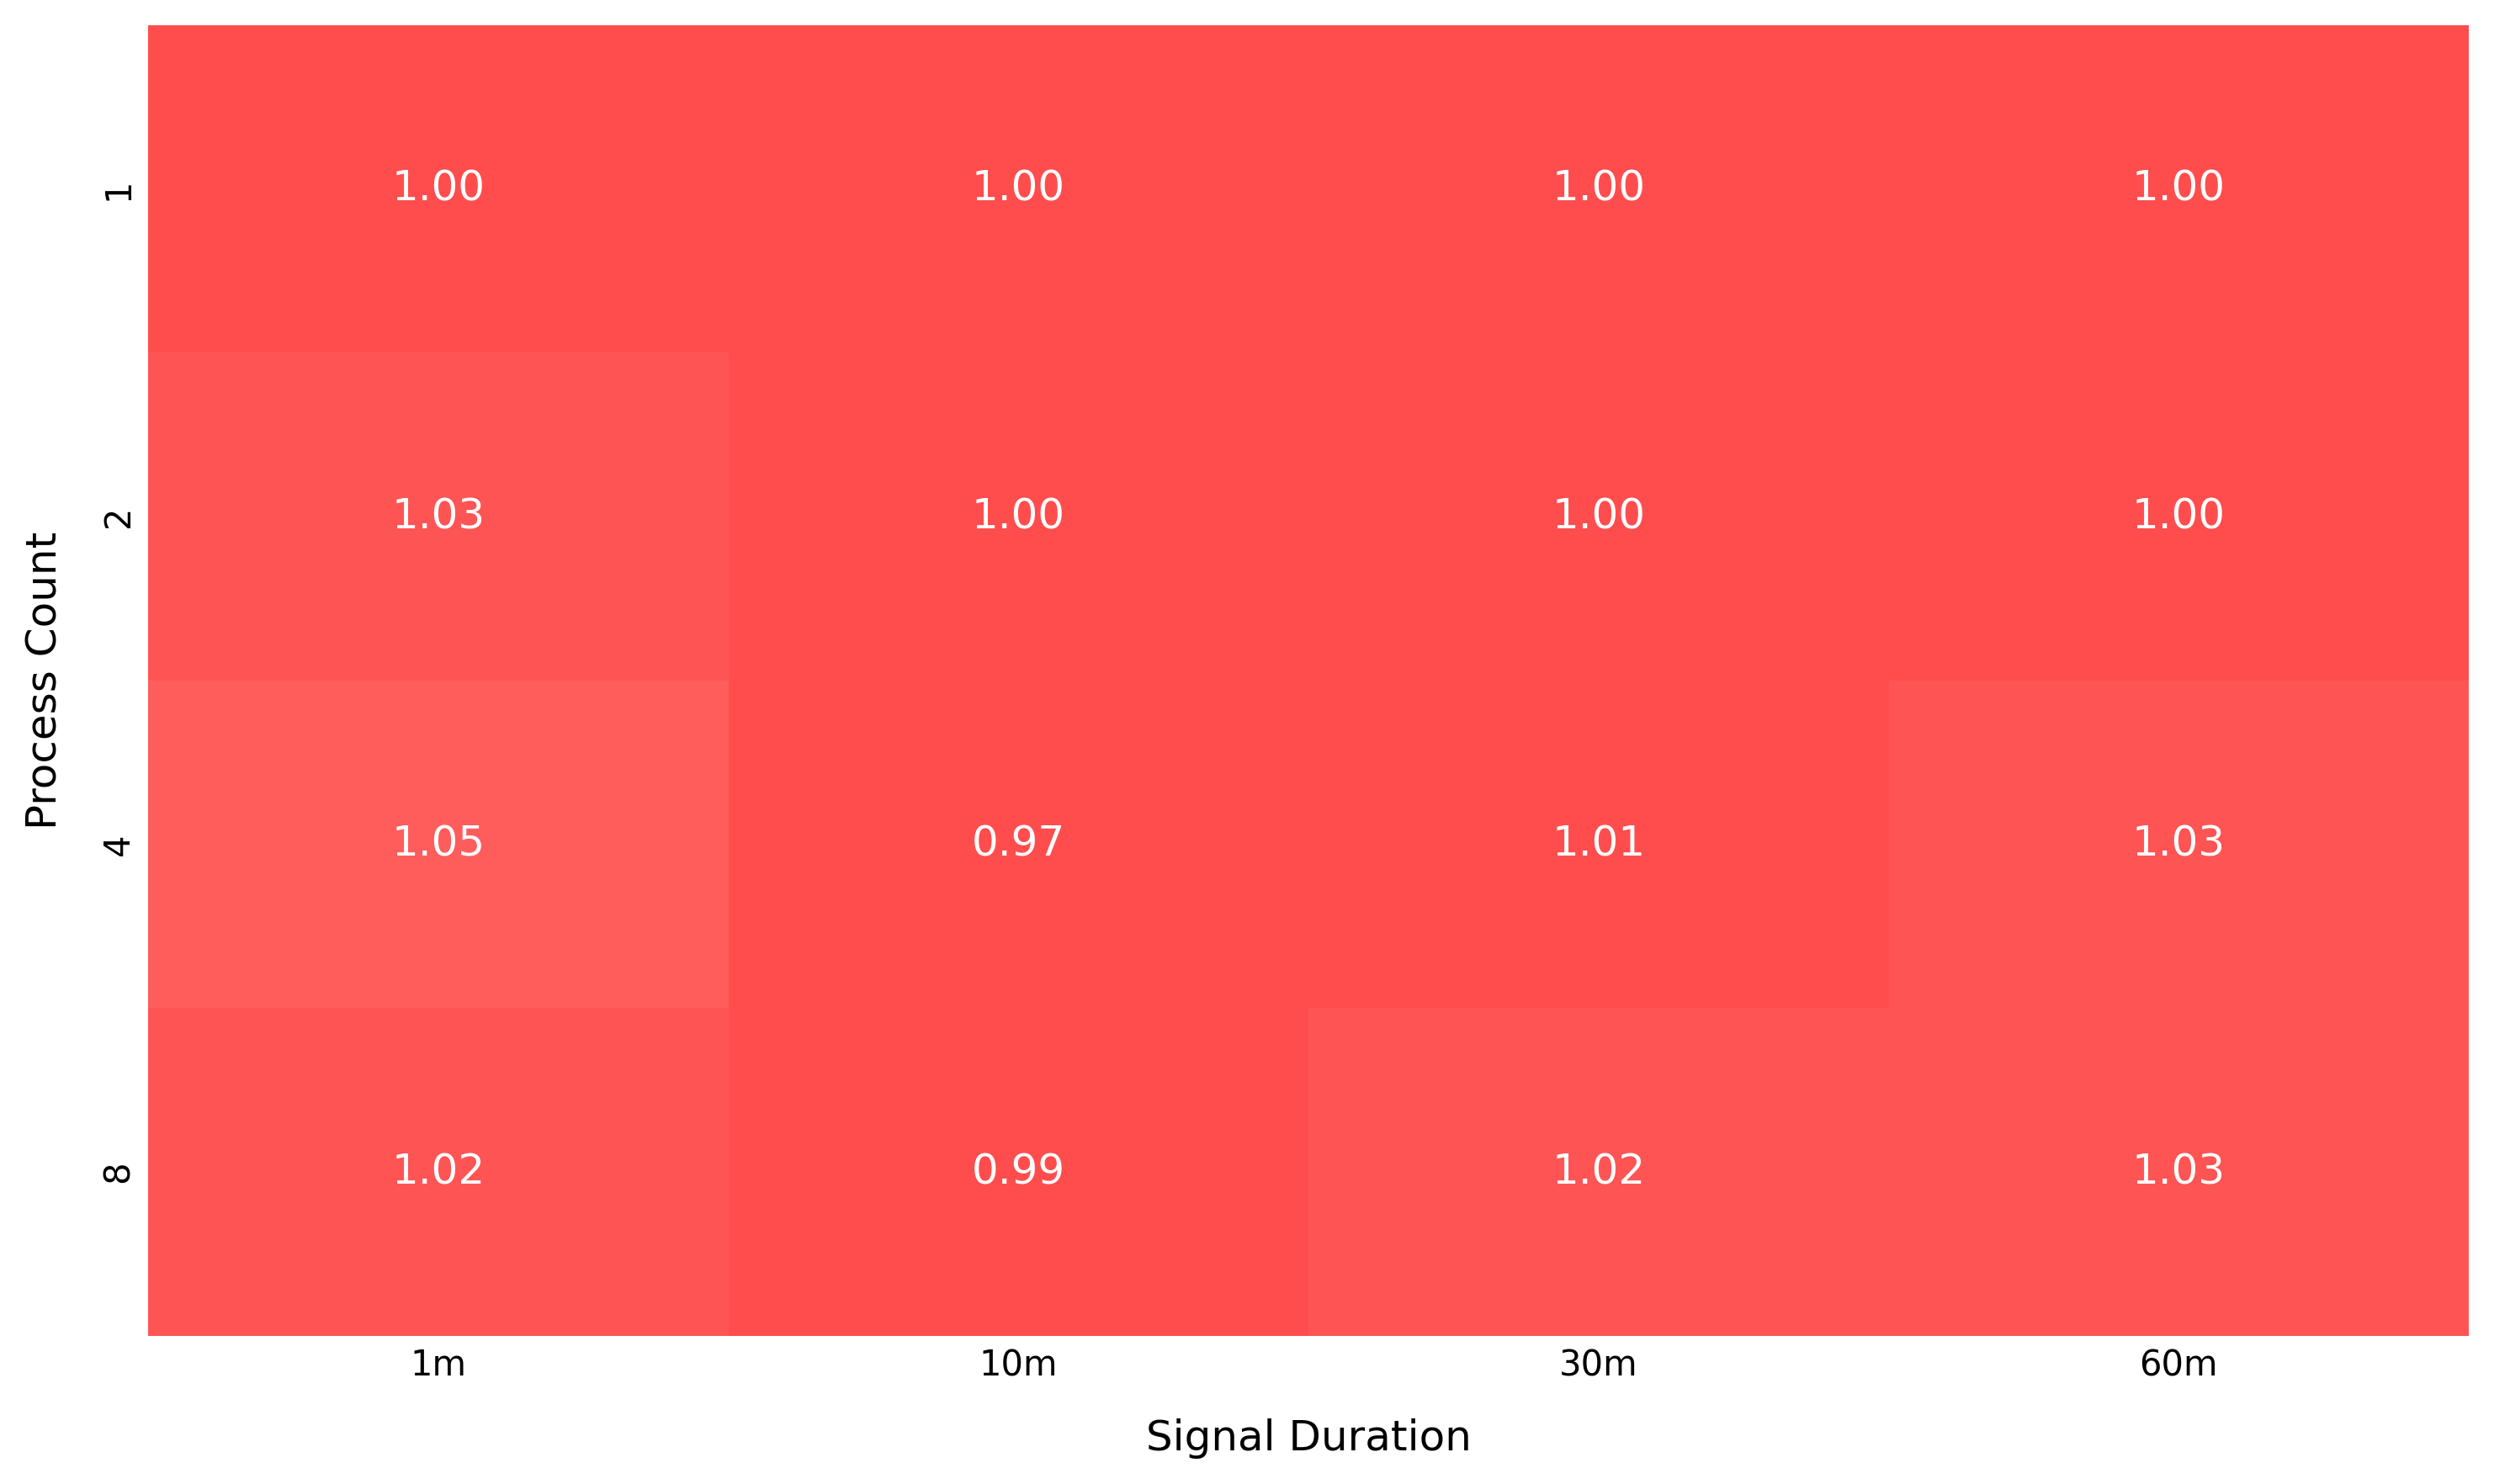
\includegraphics[scale=0.5]{figures/speedup_judas.png}
%    \caption{Heatmap of speedups with Judas compared to serial execution}
%    \label{fig:ex2judheat}
%\end{figure}